\documentclass[tikz,12pt]{standalone}

\usepackage{amsmath,amsfonts,amssymb,amsthm}
\usepackage{mathptmx}
\usepackage{tikz}
\usepackage{xcolor}

\definecolor{tblue}{RGB}{25,102,243} % blue
\definecolor{bole}{rgb}{0.8, 0.0, 0.0} % brown
\definecolor{tpink}{rgb}{0.93, 0.23, 0.51} % pink
\definecolor{tgreen}{rgb}{0.0, 0.5, 0.0} % green
\usetikzlibrary{patterns}
\usetikzlibrary{arrows}

\begin{document}

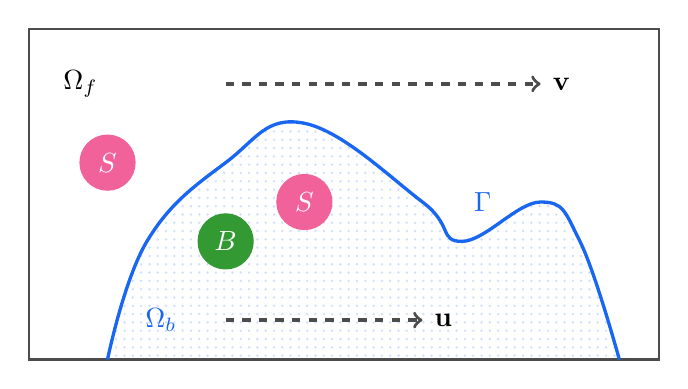
\begin{tikzpicture}

%% SETTINGS
\tikzstyle{tnode} = [
  shape=circle, 
  minimum size=5pt,
  inner sep=0pt,
  fill = tpink
]
\tikzstyle{tedge} = [
  draw = black!50,
  line width=1pt
]

% rectangle
\draw [thick, black!70]  (-3,2.2) rectangle (5,-2);
\draw [tblue,pattern=dots,pattern color=tblue!20,very thick] plot[smooth, tension=.7] coordinates {(-2,-2) (-1.5,-0.5) (-0.5,0.5) (0.5,1) (2,0) (2.5,-0.5) (3.5,0) (4,-0.5) (4.5,-2)};

% uv
% \draw [-triangle 60,dash pattern=on 3pt off 3pt,thick,black!70] plot[smooth, tension=.7] coordinates {(-0.5,1.5) (0.5,1.75) (1.5,1.5) (2.25,1.75) (3,1.5) (3.5,1.5)}; % wave
\draw [dash pattern=on 3pt off 3pt,very thick,black!70,->] (-0.5,1.5) -- (3.5,1.5);
% \draw [-triangle 60,dash pattern=on 3pt off 3pt,thick,black!70] plot[smooth, tension=.7] coordinates {(-0.5,-1.5) (0,-1.25) (0.5,-1.5) (1,-1.25) (1.5,-1.5) (2,-1.5)}; % wave
\draw [dash pattern=on 3pt off 3pt,very thick,black!70,->] (-0.5,-1.5) -- (2,-1.5);

% interface
\node[left,tblue] at (3,0) {$\Gamma$};

% fluid
\node[left] at (2.5,-1.5) {$\mathbf{u}$};
\node[left] at (4,1.5) {$\mathbf{v}$};

\draw[fill=white,tgreen!80] (-0.5,-0.5) circle (.35); % circle B
\draw[fill=white,tpink!80] (-2,0.5) circle (.35); % circle S
\draw[fill=white,tpink!80] (0.5,0) circle (.35); % circle S

\node[white] at (-2,0.5) {$S$};
\node[white] at (0.5,0) {$S$};
\node[white] at (-0.5,-0.5) {$B$};

% \draw[fill=black!80] (-2.43,1.5) circle (.35);
\node[left] at (-2,1.5) {$\Omega_f$};
% \draw[color=tblue, fill=tblue] (-1.4,-1.5) circle (.35);
\node[left,tblue] at (-1,-1.5) {$\Omega_b$};


\end{tikzpicture}

\end{document}